\documentclass[11pt, a4paper]{article}
\usepackage[T1]{fontenc}
\usepackage[utf8]{inputenc}
\usepackage[MeX]{polski}
\usepackage[polish]{babel}
\usepackage{float}
\usepackage{geometry}
\usepackage{amsmath}
\usepackage[linesnumbered,ruled]{algorithm2e}
\usepackage{graphicx}
\usepackage{caption}

\SetKw{KwDownTo}{downto}
\graphicspath{{../plots/}}

\geometry{top=1.5cm, bottom=1.5cm, right=1.5cm, left=1.5cm}


\title{Obliczenia naukowe\\Lista 4}
\author{Stanisław Woźniak}
\date{}

\begin{document}
    \maketitle
    \section{Zadanie 1.}
    \subsection{Ilorazy różnicowe}
    \subsection{Opis}
    Iloraz różnicowy jest to wartość pokazująca stosunek różnic wartości do argumentów. Jest on używany do badania przyrostu funkcji w danych punktach i najczesciej jest używany wzorem: $\frac{f(x + h) - f(x)}{h}$ gdzie $h$ jest różnicą między wybranymi punktami co przy wersji z indeksami można zastapić wzorem $\frac{f(x_{i}) - f(x_{j})}{x_{j} - x{i}}$ gdzie $i \neq j$. Natomiast uogólniony wzór:
    $$ f[x_{0},...,x_{n}] = \sum_{i = 0}^{n} \frac{f(x_{i}}{\prod_{j = 0 \and j \neq i}^{n}(x_{i} - x_{j})} $$
    Każde kolejne ilorazy różnicowe można generować ze wzoru rekurencyjnego:\\
    \centerline{$f[x_{k}] = f(x_{k})$}\\
    \centerline{$f[x_{i},...,x_{j}] = \frac{f[x_{i+1},..,x_{j}] - f[x_{i},..,x_{j-1}]}{x_{j} - x_{i}}$ gdzie $(i \neq j)$}

    Zadanie polegało na zaimplementowaniu funkcji liczącej ilorazy różnicowe mając dane węzły oraz wartości funkcji w tych węzłach. Zadanie miało zostać zrealizowane bez użycia macierzy. 
    W implementacji zostało użyte liczenie kolejnych ilorazów zgodnie ze wzorem powyżej podanym. Dzięki temu na bierząco są generowane kolejne ilorazy różnicowe, pozwalając rekurencyjnie obliczyć kolejne (w implementacji rekurencje zastąpiono odpowiednią iteracją).
    \subsection{Pseudokod}
    \begin{algorithm}[H]
        \SetKwInOut{Input}{Input}
        \SetKwInOut{Output}{Output}

        \underline{ilorazyRoznicowe} $(x, f)$\;
        \Input{$x$ - wektor węzłów, $f$ - wektor wartości funkcji w odpowiednich węzłach z $x$}
        \Output{fx - wektor ilorazów różnicowych w postaci $\{f[x_{0},...,x_{k}]: k \in \{0,...,n\}\}$}
        $n \gets length(x)$\;
        \For{$i \gets 1$ \KwTo $n$}{
            $tmp[i] \gets f[i]$\;
            \For{$k \gets 1$ \KwTo $i-1$}{
                $tmp[i-k] \gets \frac{tmp[i-k+1] - tmp[i-k]}{x[i] - x[i-k]}$\;
            } 
            $fx[i] = tmp[1]$\;
        }
        return $fx$\;
        \caption{Funkcja licząca kolejne ilorazy różnicowe}
    \end{algorithm}
    \section{Zadanie 2.}
    \subsection{Wielomian interpolacyjny Newtona}
    \subsection{Opis}
    Wielomian interpolacyjny Newtona jest to wielomian, który interpoluje podaną funkcję $f$ oraz jest postaci podanej poniżej.\\
    \centerline{\textbf{Postać Newtona wielomianu}}
    $$ N_{n}(x) = f[x_{0}] + f[x_{0}, x_{1}](x - x_{0}) + ... + f[x_{0}, x_{1}, x_{2},...,x_{n}](x - x_{0})(x - x_{1})...(x - x_{n-1})$$
    $$ N_{n}(x) = f[x_{0}] + \sum_{k=1}^{n} (f[x_{0},.., x_{k}]\prod_{j=0}^{k-1} (x - x_{j}))$$

    Zadanie polegało na zaimplementowaniu funkcji, która z pomocą algorytmu Hornera wylicza wartość wielomianu postaci Newtona.\\
    \centerline{\textbf{Uogólniony algorytm Hornera}}
    $$ w_{n}(x) = f[x_{0},...,x_{n}]$$
    $$ w_{i}(x) = f[x_{0},...,x_{i}] + (x - x_{i})w_{i+1}(x)$$
    $$i = n-1,...,0$$
    \centerline{\textbf{Związek pomiędzy wartością wielomianu Newtona a algorytmem Hornera}}
    $$ N_{n}(x) = w_{0}(x)$$

    Aby obliczyć wartość $N_{n}(x_{0})$ dla podanego $x_{0}$ powyższym algorytmem w czasie $O(n)$ rekurencja została zastąpiona odpowiednią iteracją. Użyta iteracja do obliczenia wartości został przedstawiony w poniższym pseudokodzie.

    \subsection{Pseudokod}
    \begin{algorithm}[H]
        \SetKwInOut{Input}{Input}
        \SetKwInOut{Output}{Output}

        \underline{warNewton} $(x , fx,t)$\;
        \Input{$x$ - wektor węzłów, $fx$ - wektor ilorazów różnicowych względem wektora $x$ (odpowiednio $fx[i] = f[x_{0},...,x_{i-1}]$), $t$ - argument wielomianu}
        \Output{nt - wyliczona wartość}
        $n \gets length(x)$; $nt \gets fx[n]$\;
        \For{$i \gets n-1$ \KwDownTo $1$}{
            $nt \gets  fx[i] + (t - x[i])*nt$\;
        }
        return $nt$\;
        \caption{Wyliczenie wartości wielomianu Newtona używając uogólnionego algorytmu Hornera w czasie $O(n)$}
    \end{algorithm}
    \section{Zadanie 3.}
    \subsection{Postać naturalna wielomianu interpolacyjnego Newtona}
    \subsection{Opis}
    Postać naturalna wielomianu jest to wielomian postaci: $W(x) = a_{n}x^n + ... + a_{1}x + a_{0}$. Zwijając otrzymujemy:
    $$ W(x) = \sum_{k = 0}^{n} a_{k}x^{k}$$

    Poniższy pseudokod przedstawia zaimplementowaną funkcją obliczającą współczynniki $a_{i}$ w czasie $O(n^2)$. Aby otrzymać czas kwadratowy, został użyty uogólniony algorytm Hornera do wyliczenia odpowiednich iloczynów. W tej metodzie są użyte pewne własności:
    $$ a_{n}^{(i)} = f[x_{0},...,x_{n}]$$
    $$ a_{i}^{(i)} = f[x_{0},...,x_{n}] - a_{i+1}^{(i+1)}x_{i}$$
    $$ a_{k}^{(i)} = a_{k}^{(i+1)} - a_{k+1}^{(i+1)}x_{i} $$
    \centerline{gdzie $a_{k}^{(i)}$ oznacza wspołczynnik $k$ w wielomianie $w_{i}$ z algorytmu Hornera}
    
    Używając powyższego wzoru także można użyć zależności wartości wielomianu Newtona do uogólnionego algorytmu Hornera. Z poprzedniego zadania wiadomo, że $N_{n}(x) = w_{0}(x)$, dlatego też szukane $a_{k}$ są jednoznaczne z $a_{k}^{(0)}$. W implementacji rekurencja została zastapiona odpowiednimi dwoma iteracjami względem indeksów $k$ oraz $i$, dzięki czemu czas działania wynosi $O(n^2)$;
    \subsection{Pseudokod}
    \begin{algorithm}[H]
        \SetKwInOut{Input}{Input}
        \SetKwInOut{Output}{Output}

        \underline{naturalna} $(x , fx)$\;
        \Input{$x$ - wektor węzłów, $fx$ - wektor ilorazów różnicowych względem wektora $x$ (odpowiednio $fx[i] = f[x_{0},...,x_{i-1}]$)}
        \Output{a - wektor zawierający współczynniki postaci naturalnej gdzie $a[i] = a_{i-1}$}
        $n \gets length(x)$; $a[n] = fx[n]$\; 
        \For{$i \gets n-1$ \KwDownTo $1$}{
            $a[i] \gets fx[i]$\;
            \For{$k \gets i$ \KwTo $n-1$}{
                $a[k] \gets a[k] - x[i]a[k+1]$\;
            }
        }
        return $a$\;
        \caption{Obliczenie współczynników wielomianu interpolacyjnego postaci naturalnej w czasie $O(n^2)$}
    \end{algorithm}
    \section{Zadanie 4.}
    \subsection{Rysowanie wykresów}
    \subsection{Opis}
    Zadanie polegało na zaimplementowaniu funkcji, która rysowałaby wykres funkcji oraz wykres wielomianu interpolacyjnego używając implementacji z poprzednich zadań. Funkcja rysująca polegała na stworzeniu dwóch wektorów. Do tego zostały użyte dane wejściowe, tzn: funkcji $f$, przedziału rysowania oraz liczby całkowitej $n$, która odpowiada stopniu wielomianu interpolacyjnego. Na początku funkcja generuje $n+1$ węzłów, które są w równej odległości od siebie, następnie wylicza dla podanych węzłów odpowiadające im wartości. Następnie wygenerowane wektory węzłow oraz ich wartości zostały przekazane do zaimplementowanej wcześniej funkcji $ilorazyRoznicowe$ dzięki której wylicza tablice ilorazów różnicowych postaci $\{f[x_{0},...,x_{i}]: i \in \{0,...,n\}\}$. Następnie generuje w podobny sposób co zostały generowane węzły, punkty, które zostaną nałożone na wykres z tą różnicą, że jest ich znacznie więcej, aby rysunek był dokładniejszy. Dla wykresu wielomianu interpolacyjnego, do obliczenia wartości danych węzłów została użyta wcześniej zaimplementowana funkcja $warNewton$. Ostatnim krokiem jest ostatecznie nałożenie wyliczonych danych na wykres.
    \subsection{Pseudokod}
    \begin{algorithm}[H]
        \SetKwInOut{Input}{Input}
        \SetKwInOut{Output}{Output}

        \underline{rysujNnfx} $(f, a, b, n)$\;
        \Input{$f$ - dana funkcja, $a,b$ - przedział rysowania, $n$ - stopień wielomianu interpolacyjnego}
        \Output{wykres}
        $h \gets \frac{b-a}{n}$\;
        \For{$k \gets 0$ \KwTo $n$}{
            $xk \gets a + kh$\;
            $append(x, xk)$; $append(values, f(xk))$\;
        }
        $fx \gets ilorazyRoznicowe(x, values)$\;

        $temporaryX \gets x$\;
        $n \gets$ \textit{wybrana dokłądność}\;
        \textit{Powtórzenie pętli z linii 3. z tą różnicą, że zamiast $f(xk)$ używa się $warNewton(temporaryX, fx, xk)$}
        \\
        \textit{Nałożenie wygenerowanych wartości na wykresy}\\
        \caption{Funkcja rysująca wykres funkcji oraz wielomianu interpolacyjnego stopnia n}
    \end{algorithm}
    \section{Zadanie 5.}
    \subsection{Problem}
    W zadaniu został przedstawiony problem polegający na porównaniu dwóch funkcji z ich wielomianami interpolacyjnymi stopnia n używając powyższych funkcji oraz podanych przedziałów rysowania.\\
    \\
    $n \in \{5, 10, 15\}$\\
    $a(x) = e^{x}$, przedział rysowania: $[0,1]$\\
    $b(x) = x^2\sin{x}$, przedział rysowania: $[-1, 1]$
    \subsection{Wyniki}
    Objaśnienie wykresów:\\
    y1 (kolor niebieski) - graficzne przedstawienie wyliczonyego wielomianu interpolacyjnego.\\
    y2 (kolor czerwony) - graficzne przedstawienie podanej funkcji.
    \begin{figure}[H]
        \captionsetup{labelformat = empty}
        \begin{minipage}{0.5\textwidth}
            \centerline{\textbf{Wykresy funkcji a:}}
            \caption{$n=5$}
            \centering
            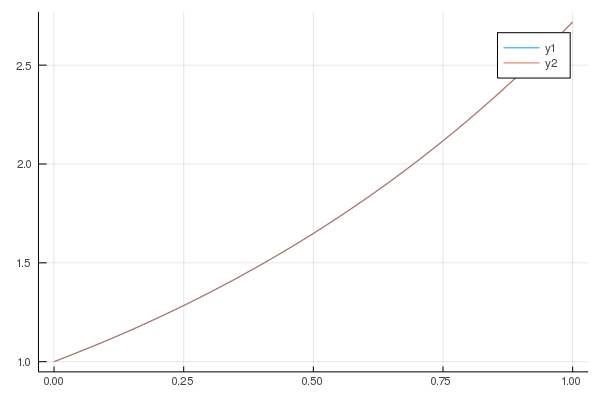
\includegraphics[width=\linewidth]{plot-5_a_n5}
        \end{minipage}
        \begin{minipage}{0.5\textwidth}
            \centerline{\textbf{Wykresy funkcji b:}}
            \caption{$n=5$}
            \centering
            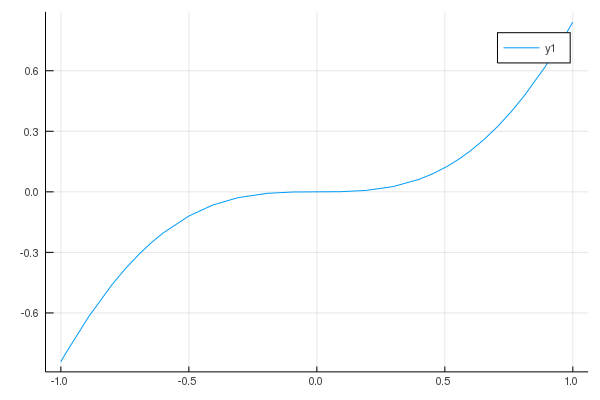
\includegraphics[width=\linewidth]{plot-5_b_n5}
        \end{minipage}

        \begin{minipage}{0.5\textwidth}
            \caption{$n=10$}
            \centering
            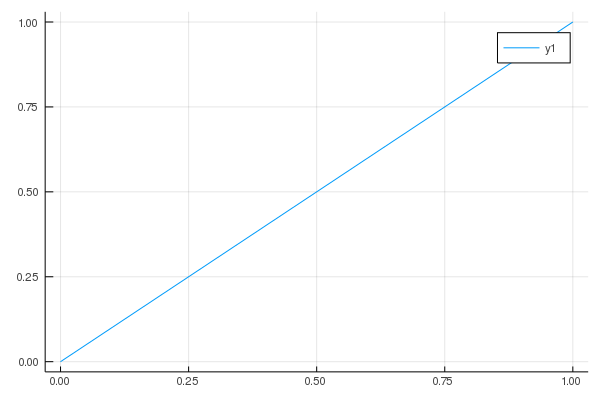
\includegraphics[width=\linewidth]{plot-5_a_n10}
        \end{minipage}
        \begin{minipage}{0.5\textwidth}
            \caption{$n=10$}
            \centering
            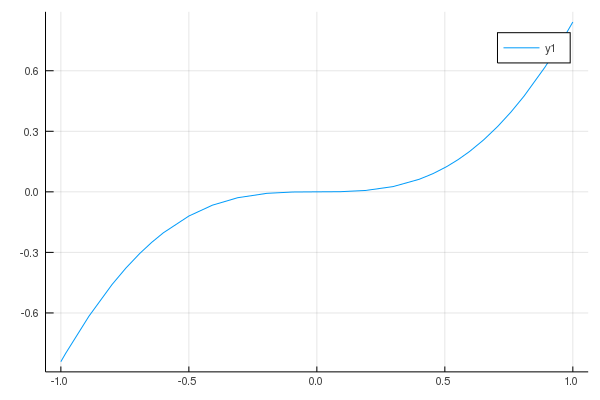
\includegraphics[width=\linewidth]{plot-5_b_n10}
        \end{minipage}
        
        \begin{minipage}{0.5\textwidth}
            \caption{$n=15$}
            \centering
            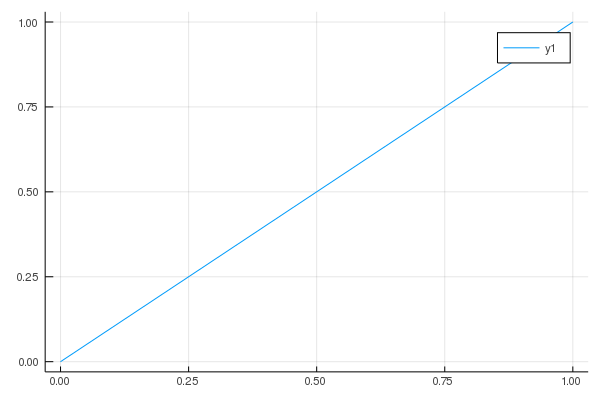
\includegraphics[width=\linewidth]{plot-5_a_n15}
        \end{minipage}
        \begin{minipage}{0.5\textwidth}
            \caption{$n=15$}
            \centering
            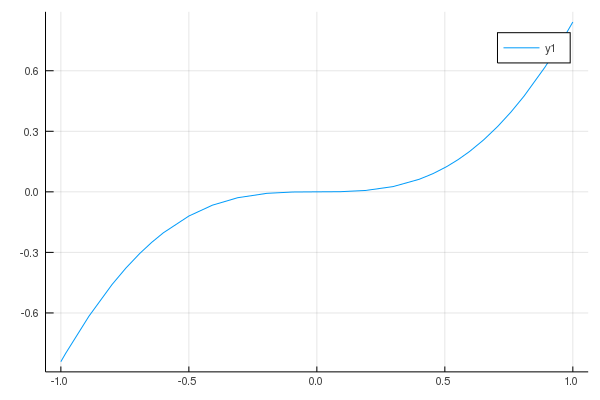
\includegraphics[width=\linewidth]{plot-5_b_n15}
        \end{minipage}
    \end{figure}
    \subsection{Wnioski}
    Obserwując powyższe wykresy można zauważyć zgodność wielomianu interpolacyjnego z pierwotną funkcją. Oznacza to, że dla podanych funckji dobranie węzłów równoodległych od siebie jest odpowiednim rozwiązaniem do uzyskania szukanego przybliżenia wielomianem interpolacyjnym. Dzieje się to dlatego, że obie z funkcji są funkcjami gładkimi, co oznacza, że istnieją ich pochodne wszystkich rzędów oraz są one ciągłe. 

    \section{Zadanie 6.}
    \subsection{Problem}
    Problemem w zadaniu było pokazanie na wykresach podane funkcjie oraz ich wielomiany interpolacyjne stopnia n.\\
    \\
    $n \in \{5, 10, 15\}$\\
    $a(x) = |x|$, przedział rysowania: $[-1,1]$\\
    $b(x) = \frac{1}{1 + x^2}$, przedział rysowania: $[-5, 5]$
    \subsection{Wyniki}
    Objaśnienie wykresów:\\
    y1 (kolor niebieski) - graficzne przedstawienie wyliczonyego wielomianu interpolacyjnego.\\
    y2 (kolor czerwony) - graficzne przedstawienie podanej funkcji.
    \begin{figure}[H]
        \captionsetup{labelformat = empty}
        \begin{minipage}{0.5\textwidth}
            \centerline{\textbf{Wykresy funkcji a:}}
            \caption{$n=5$}
            \centering
            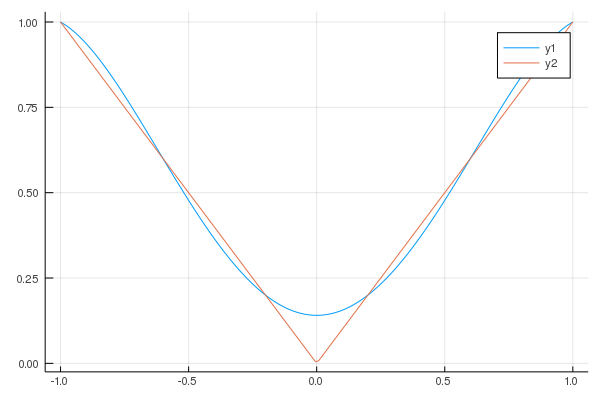
\includegraphics[width=\linewidth]{plot-6_a_n5}
        \end{minipage}
        \begin{minipage}{0.5\textwidth}
            \centerline{\textbf{Wykresy funkcji b:}}
            \caption{$n=5$}
            \centering
            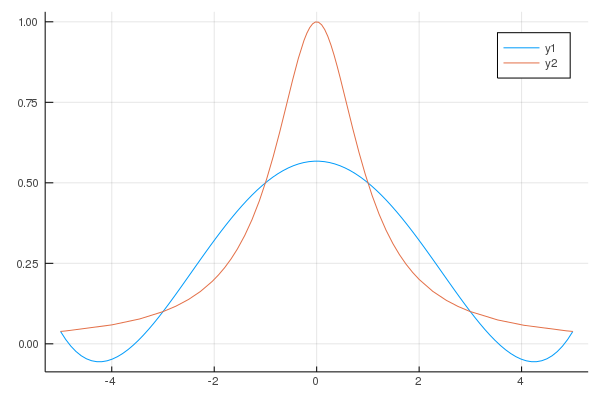
\includegraphics[width=\linewidth]{plot-6_b_n5}
        \end{minipage}

        \begin{minipage}{0.5\textwidth}
            \caption{$n=10$}
            \centering
            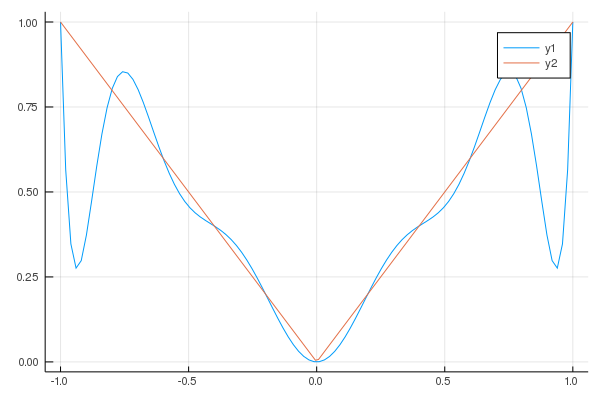
\includegraphics[width=\linewidth]{plot-6_a_n10}
        \end{minipage}
        \begin{minipage}{0.5\textwidth}
            \caption{$n=10$}
            \centering
            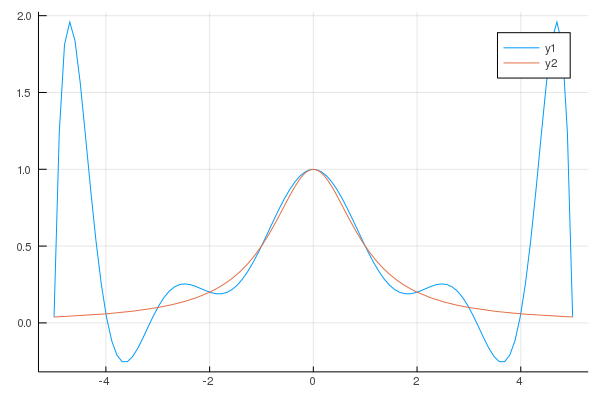
\includegraphics[width=\linewidth]{plot-6_b_n10}
        \end{minipage}
        
        \begin{minipage}{0.5\textwidth}
            \caption{$n=15$}
            \centering
            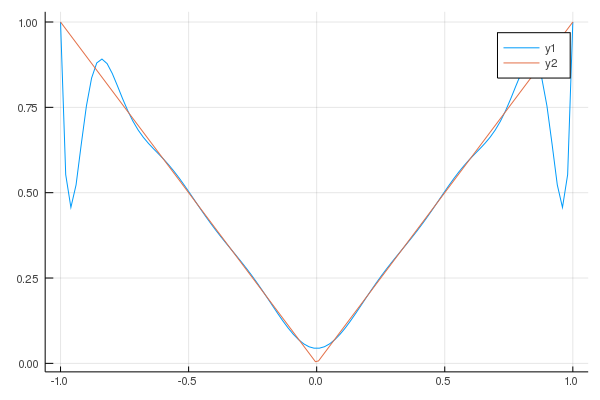
\includegraphics[width=\linewidth]{plot-6_a_n15}
        \end{minipage}
        \begin{minipage}{0.5\textwidth}
            \caption{$n=15$}
            \centering
            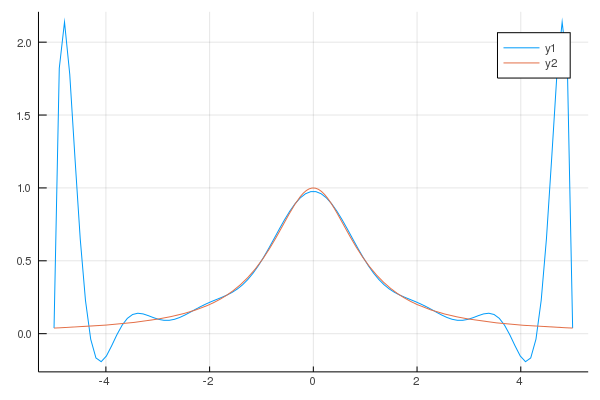
\includegraphics[width=\linewidth]{plot-6_b_n15}
        \end{minipage}
    \end{figure}
    \subsection{Wnioski}
    Analizując powyższe wykresy od razu można zauważyć, że wielomian interpolujący jest rozbiezny względem funkcji. Rozbiezność najwidoczniejsza jest przy końcach przedziału. Także dla większej ilości węzłów rozbieżność jest większa. Taki efekt nazywa się efeketem Rungego. Zachowanie to jest częste dla wielomianów interpolacyjnych wysokiego stopnia kiedy węzły są równoodległe od siebie. W przypadku funkcji $a$ dzieje się to dlatego, że nie jest ona różniczkowalna i nie istnieje jej pochodna. Oznacza to, że funkcja $a$ odbiega znaczaco od funkcji gładkiej, co jest jednym z przypadków kiedy występuj efekt Rungego. Natomiast funkcja $b$ jest gładka oraz ciągła, przez co można zakładać, że wraz z wzrostem liczby węzłów wielomian bedzie przybliżał się do interpolowanej funkcji lecz tak sie nie dzieje. Jest to związane tym, że węzły są w równej odległości od siebie, więc na krawędziach przedziału, gdzie daną funkcje trudniej przybliżyć jest tyle samo węzłów co przy środku przedziału. Można pomyśleż, że aby temi zapobiec nalezy dołożyć odpowiednią liczbe węzłów przy końcach przedziału. Takie zachowanie jest typowe dla wielomianów Czebyszewa, które posiadają rozmieszczenie węzłów zagęszczone przy końcach przedziału. Rozwiązanie to zapobiega rozbieżności wielomianu interpolacyjnego względem interpolującej funkcji.

\end{document}
